\section{Theory}
\subsection{The Fabry-Perot interferometer}\label{sec:fabry_perot}

The Fabry-Perot interferometer, also known as an optical cavity, is generally comprised of two reflective optical elements, hereafter refered to as mirrors. In the following we assume a plane-plane configuration for two lossless mirrors and a plane-wave at normal incidence for the incoming field, as sketched in figure \ref{fig:planar_fabry-perot}. 

\begin{figure}[h!]
    \centering
    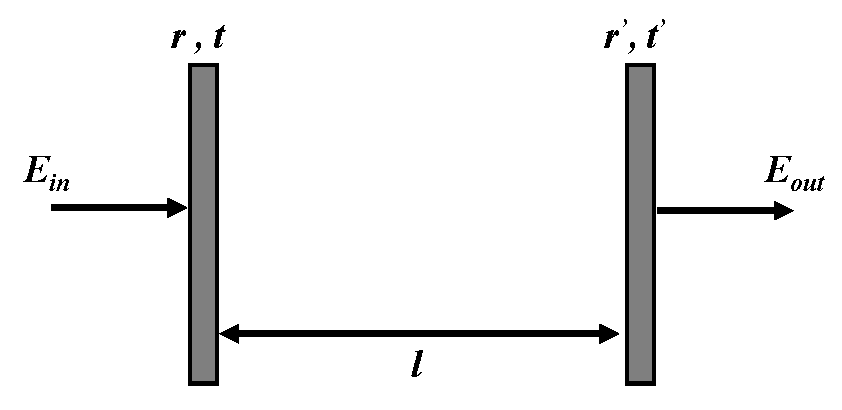
\includegraphics[width=0.6\textwidth]{figures/planar_fabry_perot.pdf}
    \caption{Sketch of a planar Fabry-Perot cavity.}
    \label{fig:planar_fabry-perot}
\end{figure}

The two mirrors are described by each their respective reflectivity \emph{r} and transmission \emph{t} and are placed parallel at a distance \emph{l} from each other. The field at the second mirror, i.e. the transmitted field $E_{out}$ can then be described as a function of the field at the first mirror, i.e. the incident field $E_{in}$. The Fabry-Perot cavity furthermore gives rise to so-called eigenstates related to it's length \emph{l}, derived from considering the path difference between succesive parallel beams through the cavity. Any allowed mode inside the cavity, and thus transmitted, must fulfill the brightness condition $2l = m \lambda$, where $\lambda$ is the wavelength of the incident field and $m=1,2,3,...$ is a positive integer.\cite{Eichhorn}\cite{Pedrotti}

\subsubsection{Transmission}

In order to determine the transmission throught the Fabry-Perot cavity, we once again consider the configuration in figure \ref{fig:planar_fabry-perot}. It is further, initially, assumed that the mirrors are both lossless, such that
\begin{equation}
    |r|^2 + |t|^2 = |r^{\prime}|^2 + |t^{\prime}|^2 = 1.
    \label{eq:lossless_condition}
\end{equation}

This means that all losses, e.g. due to absorption or scattering, are neglected. 

In order to formulate $E_{out}$ in terms of $E_{in}$, we first consider the incident field as a propagating plane-wave
\begin{equation}
    E_{in} = E_{0,in} e^{ik},
\end{equation}

where $k = 2 \pi / \lambda$ is the wave number and $E_{0,in}$ is the amplitude of the field. We then consider $E_{out}$ to be comprised of contributions for each roundtrip inside the cavity. This can be written as an infinite geometrical series given as
\begin{equation}
    \begin{split}
        E_{out} & = tt^{\prime} E_{0,in} e^{ik} + tt^{\prime} E_{0,in} e^{ik} rr^{\prime} e^{i\delta}\\&+ tt^{\prime} E_{0,in} e^{ik} \left(rr^{\prime} e^{i\delta}\right)^2 + tt^{\prime} E_{0,in} e^{ik} \left(rr^{\prime} e^{i\delta}\right)^3 + ...\\& = tt^{\prime} E_{0,in} e^{ik} \sum^{\infty}_{m=0}\left( rr^{\prime}e^{i\delta} \right)^m
    \end{split}
    \label{eq:transmission_as_geometric_series}
\end{equation}
where $\delta = 2kl$. The first term of the series corresponds to a direct transmission through the cavity, and each term thereafter corresponds to the respective contribution to the transmission after the $m'th$ round trip. 

By evaluating the series it is seen that it converges to the final expression for the transmitted field through a planar Fabry-Perot cavity
\begin{equation}
    E_{out} = E_{0,in}\frac{tt^{\prime} e^{i\delta /2}}{1 - rr^{\prime} e^{i\delta}}.
    \label{eq:fabry_perot_trans}
\end{equation}

The intensity of the transmission is now taken as the square of the norm of the field amplitude $|E_{out}|^2$ and normalizing with respect to the incident field intensity $|E_{0,in}|^2$. We arrive at an expression for the transmission intensity which is recognized to be given on the form of an \emph{Airy function}\cite{Pedrotti}
\begin{equation}
    T = \frac{|E_{out}|^2}{|E_{0,in}|^2} = \left|\frac{tt^{\prime}e^{i\delta/2}}{1 - rr^{\prime}e^{i \delta}}\right|^2 = \frac{(1-|r|^2)(1-|r^{\prime}|^2)}{(1-|rr^{\prime}|)^2 + 4|rr^{\prime}|sin^2(\delta)},
    \label{eq:airy_function}
\end{equation}
where $\delta$ is the phase shift associated with each round trip inside the cavity.

\begin{figure}[h!]
    \centering
    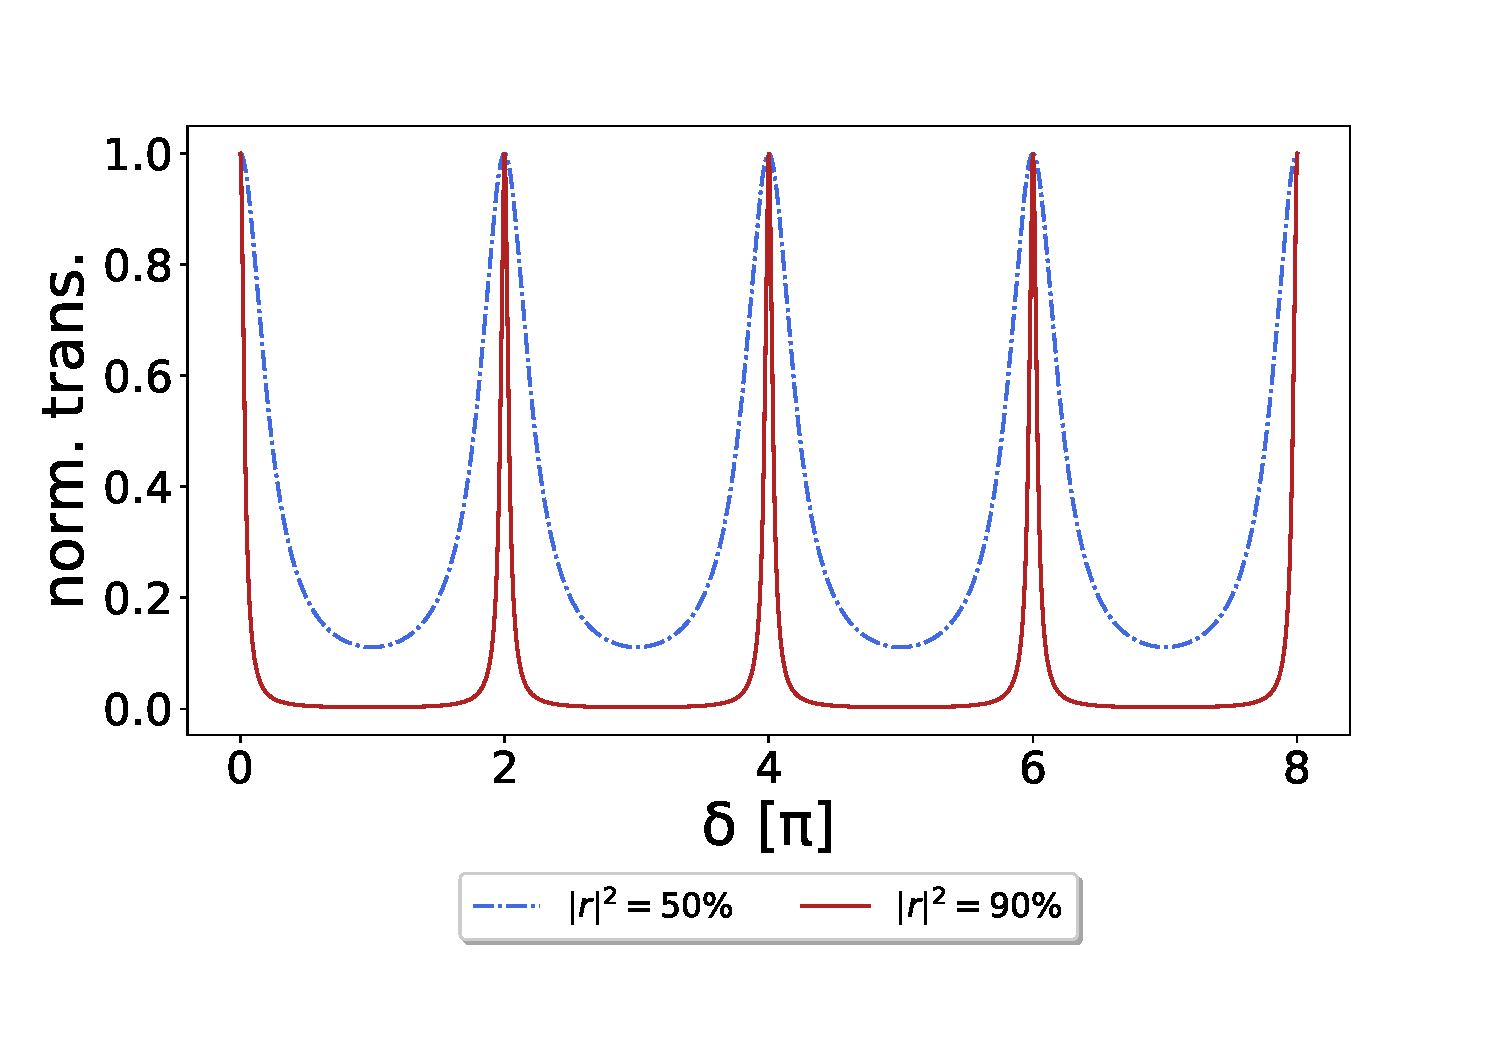
\includegraphics[width=0.7\textwidth]{figures/fabry_perot_high_and_low_finesse.pdf}
    \caption{The red line shows the transmission spectrum of a \emph{high} finesse Fabry-Perot cavity of reflectivity $|r|^2 = 0.90$, while the blue dashed line shows the transmission spectrum of a \emph{low} finesse cavity with reflectivity $|r|^2 = 0.50$.}
    \label{fig:fabry_perot_trans}
\end{figure}

Figure \ref{fig:fabry_perot_trans} displays the Airy function in eq. (\ref{eq:airy_function}), of a lossless cavity of reflectivities $r^{\prime} = r$, as a function of $\delta$ in units of $\pi$. The function is plotted for the cases of $|r|^2 = 50 \%$, shown in blue, and $|r|^2 = 90 \%$, shown in red. It is readily seen that the transmission is maximized for $\delta = n 2 \pi$ and that the two cases shown differ significantly as the red profile is much narrower than the blue. The red profile is hence said to have a higher \emph{finesse} $\mathcal{F}$ than the blue profile. The finesse is defined as
\begin{equation}
    \mathcal{F} \equiv \frac{FSR}{\delta_{\lambda}},
    \label{eq:finesse_definition}
\end{equation}
where $FSR$ is the so-called \emph{Free Spectral Range} indicating the spectral distance between two peaks and $\delta_{\lambda}$ refers to the \emph{Full Width at Half Maximum (FWHM)} which, as the name suggests, is the linewidth defined at a normalized transmission $T=1/2$, i.e. at half the maximum value. 

Considering the Airy function in eq. (\ref{eq:airy_function}) for the high finesse case where $|r|^2 = |r^{\prime}|^2 \rightarrow 1$ we furthermore see that each individual peak closely resembles a Lorentzian distribution. 

\subsubsection{Varying the cavity length}

In order to relate the resonance transmission profile to the length of the cavity we first consider the frequencies at which the cavity is resonant, with respect to the incident light, given as
\begin{equation}
    \nu_n = n \frac{c}{2l},
    \label{eq:resonance_freq}
\end{equation}
where $c$ is the speed of light, $n$ is a positive integer refering to the order of the resonance frequency and $l$ is the cavity length. This corresponds to resonance occuring at times related to each round trip inside the cavity. 

Since the FSR is defined as the spectral distance between each peak, it follows from eq. (\ref{eq:resonance_freq}) that it can be be expressed in units of frequency as 
\begin{equation}
    FSR_{\nu} = \frac{c}{2l},
    \label{eq:FSR_vs_cavity_length}
\end{equation}
and the corresponding linewidth, or FWHM, $\delta_{\nu}$ is then given as
\begin{equation}
    \delta_{\nu} = \frac{1}{2 \pi} \frac{|t|^2 + |t^{\prime}|^2}{\tau},
\end{equation}
where $\tau = 2l/c$ is the round trip time in seconds. 

Finally, considering the definition of the finesse from eq. (\ref{eq:finesse_definition}) it can be shown that
\begin{equation}
    \mathcal{F} \equiv \frac{FSR_{\nu}}{\delta_{\nu}} = \frac{2 \pi}{|t|^2 + |t^{\prime}|^2},
    \label{eq:lossless_finesse}
\end{equation}
where the finesse is now defined in terms of the total cavity transmission at resonance. 

Note here that the relation between the FSR and the cavity length $l$ is clearly shown in eq. (\ref{eq:FSR_vs_cavity_length}), and figure \ref{fig:fabry_perot_FSR_comparison} furthermore shows transmission spectra underlining the effect of changing the cavity length. 

\begin{figure}[h!]
    \centering
    \begin{subfigure}[b]{0.49\textwidth}
        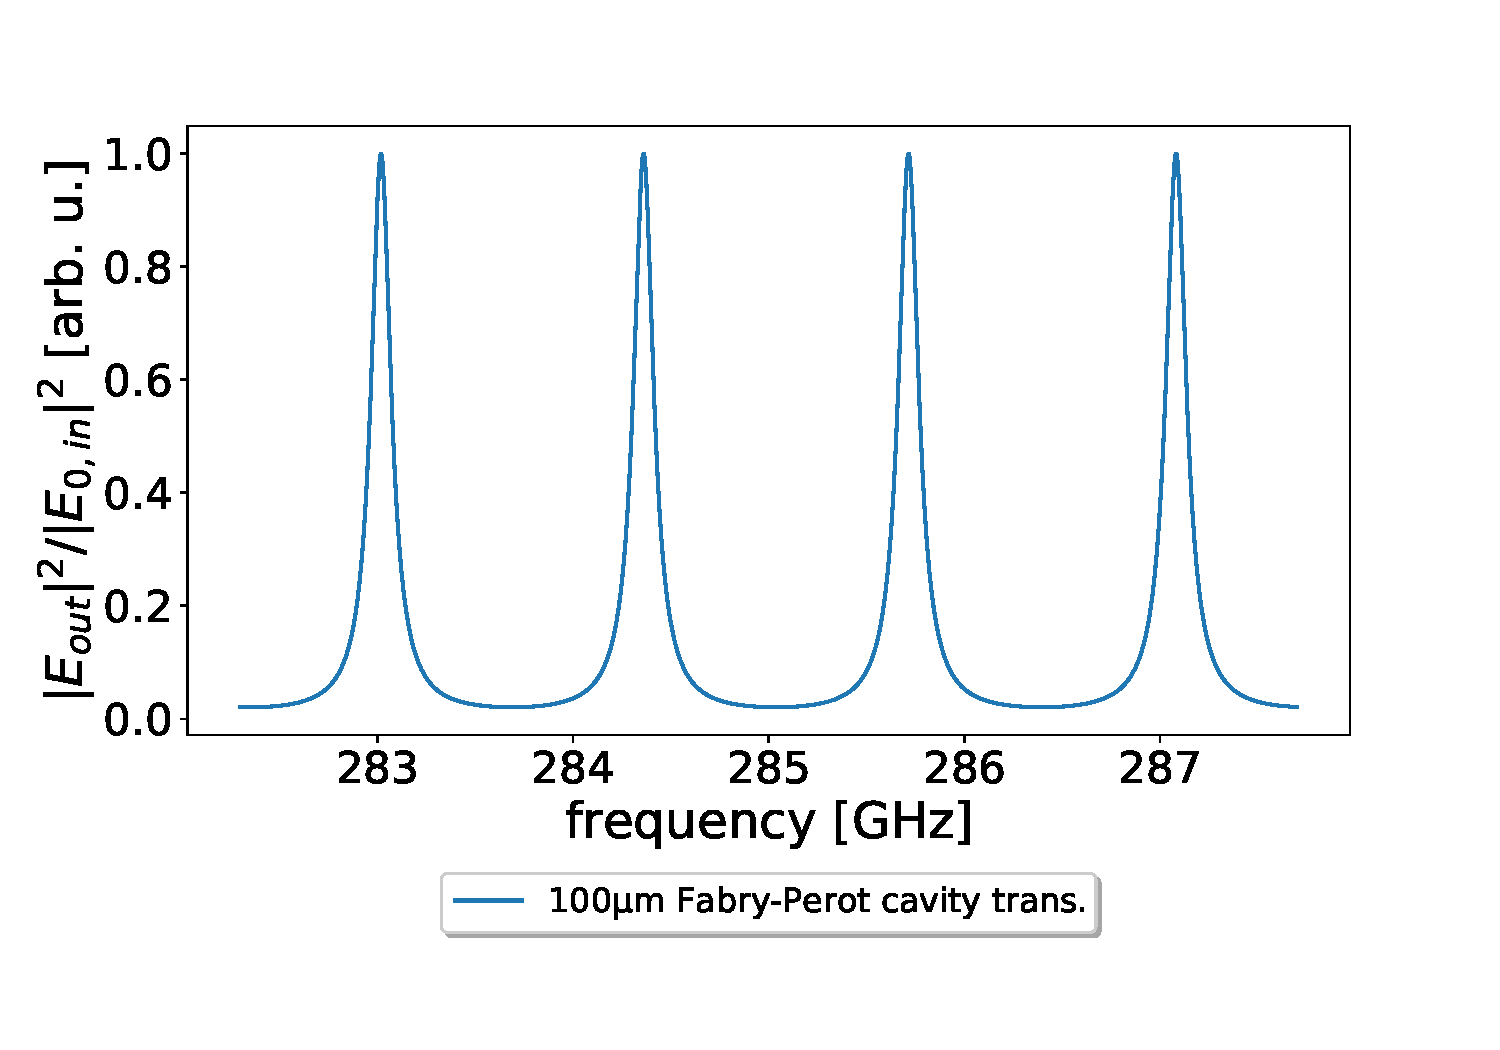
\includegraphics[width=\textwidth]{figures/100um_fabry_perot_trans_vs_freq.pdf}
        \caption{}
    \end{subfigure}
    \begin{subfigure}[b]{0.49\textwidth}
        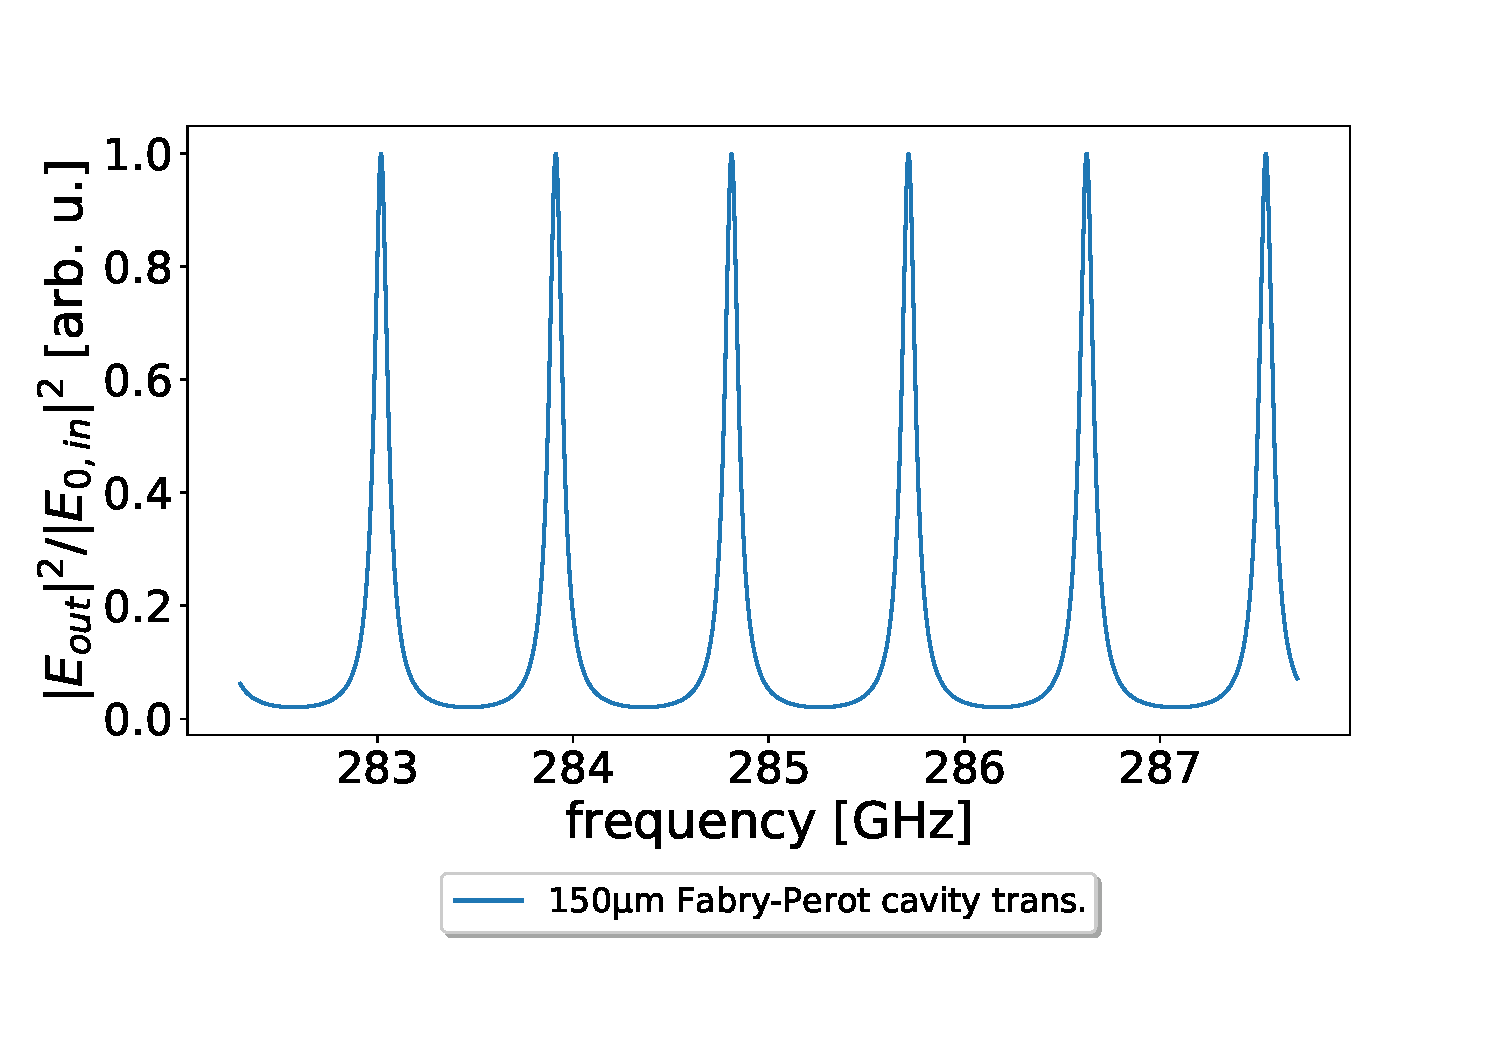
\includegraphics[width=\textwidth]{figures/150um_fabry_perot_trans_vs_freq.pdf}
        \caption{}
    \end{subfigure}
    \caption{(a) shows the transmission spectrum of a Fabry-Perot cavity of length $l \approx 100 \mu m$ as a function of the frequency $\nu$, while (b) shows the transmission spectrum of a cavity of length $l \approx 150 \mu m$ for the same range of frequencies. Note here how the FSR is inversely proportional to the cavity length.}
    \label{fig:fabry_perot_FSR_comparison}
\end{figure}

\subsubsection{Varying the incident wavelength}

In order to simplify the Airy function in eq. (\ref{eq:airy_function}) we introduce the so-called \emph{coefficient of finesse} $F$, which is a function only of the mirror reflectivites, given as
\begin{equation}
    F = \frac{4 |rr^{\prime}|}{(1-|rr^{\prime}|)^2}.
\end{equation}

The coefficient of finess $F$ is not to be confused with the finesse $\mathcal{F}$. While the finesse is related to the sharpness of the transmission peaks, the coefficient of finesse refers to the contrast of the peaks in the sense that the difference between the minimum and maximum transmitance level increases with $F$. The coefficient of finesse is related to the finesse as 
\begin{equation}
    \mathcal{F} = \frac{\pi}{2} \sqrt{F}.
\end{equation}

Rewriting the Airy function in terms of the coefficient of finesse yields
\begin{equation}
    T_{\lambda} = \frac{1}{1+ F sin^2 \left(\delta / 2\right)},
    \label{eq:simplified_airy_function}
\end{equation}
where the round trip phase shift $\delta$ is related to the wavelength $\lambda$ of the incident light by
\begin{equation}
    \delta = 2kl = \frac{4 \pi l }{\lambda},
\end{equation}
as $k = 2 \pi / \lambda$ is the incident wave number.

Re-writing the general cavity brightness condition, it can easily be shown that the resonant wavelengths for a cavity at normal incidence are given as
\begin{equation}
    \lambda_n = \frac{2l}{n},
\end{equation}
where $n=1,2,3,...$ is a positive integer refering to the order of the resonance. 

Since $\nu = c / \lambda$, the relation between the linewidth in wavelength space $\delta_{\lambda}$ and the one in frequency space $\delta_{\nu}$ is non-linear. Therefore one does not simply make the aforementioned substitution in order to relate them. It can however be shown that their respective expressions differ by a factor of $\lambda^2/c$, and the linewidth when varying the wavelength is thus given as
\begin{equation}
    \delta_{\lambda} = \frac{\lambda^2}{c} \cdot \delta_{\nu} = \frac{\lambda^2}{4 \pi l} (|t|^2 + |t^{\prime}|^2).
\end{equation}
Finally we consider the definition for the finesse $\mathcal{F}$ and the expression given in eq. (\ref{eq:lossless_finesse}), in order to show that the $FSR$ in wavelength space is given as 
\begin{equation}
    FSR_{\lambda} \equiv \delta_{\lambda} \cdot \mathcal{F} =  \frac{\lambda^2}{2l}.
\end{equation}
Figure \ref{fig:airy_trans_vs_wavelength} shows an example of the Airy function given in eq. (\ref{eq:simplified_airy_function}) as a function of the wavelength for a Fabry-Perot cavity of reflectivies $|r|^2 = |r^{\prime}|^2 = 90\%$ and length $l=100 \mu m$.

\begin{figure}[h!]
    \centering
    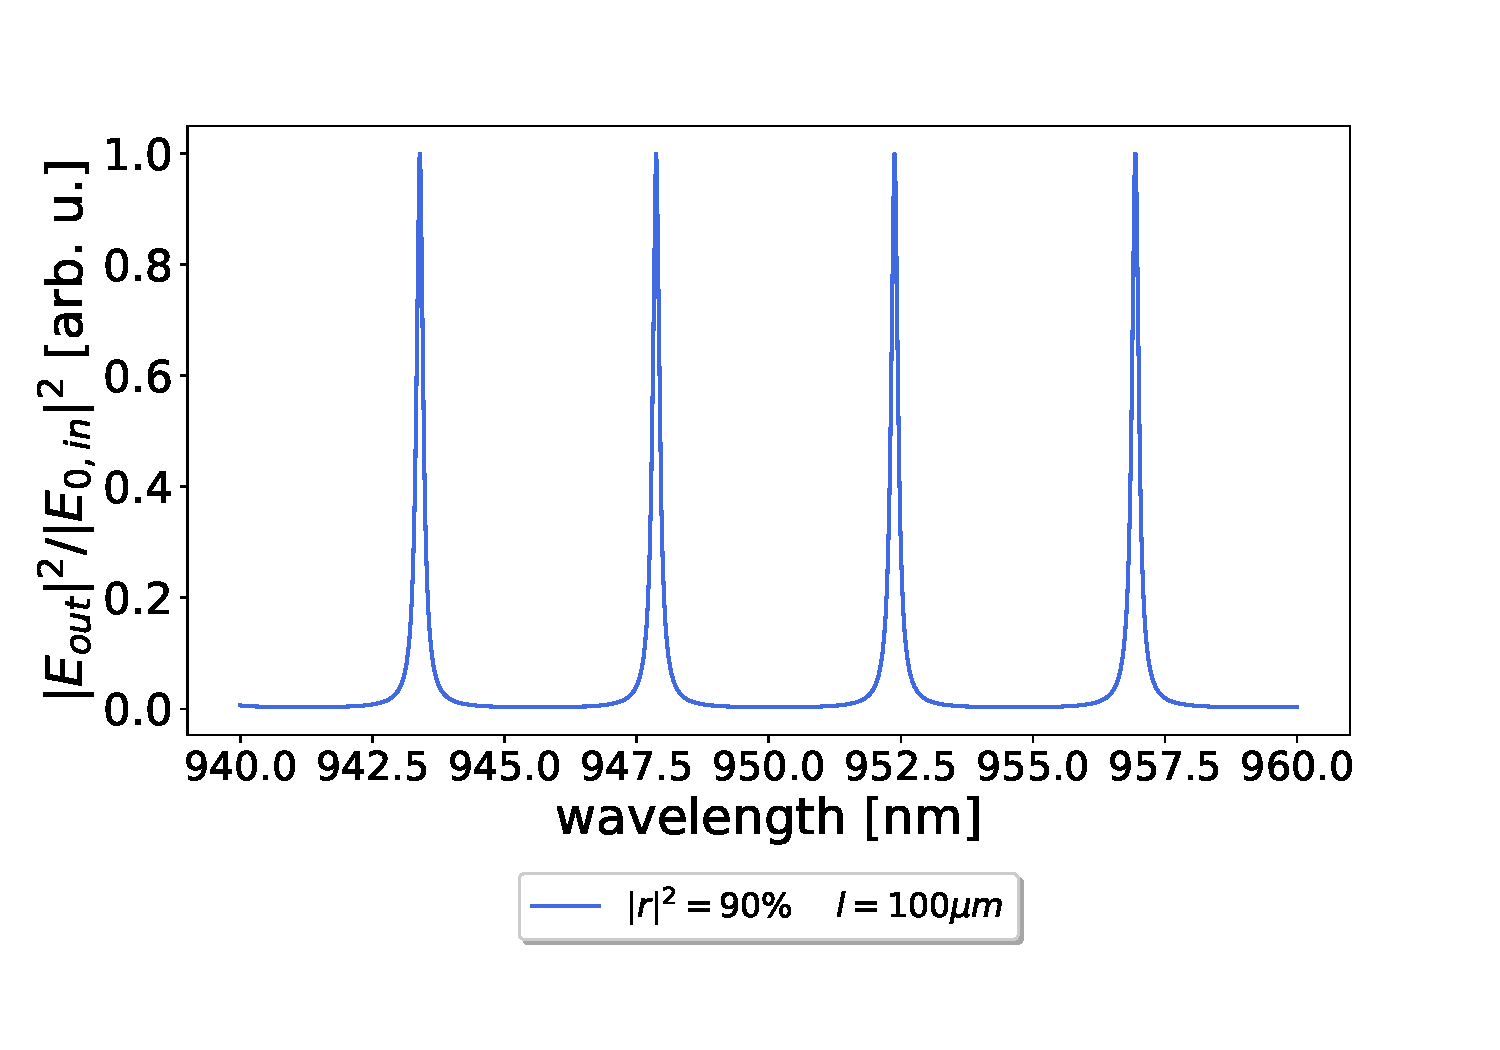
\includegraphics[width=0.7\textwidth]{figures/airy_function_vs_wavelength.pdf}
    \caption{The Fabry-Perot transmission function on the form of an Airy function as seen in eq. (\ref{eq:simplified_airy_function}) as a function of the incident wavelength.}
    \label{fig:airy_trans_vs_wavelength}
\end{figure}

\subsubsection{Cavity losses}

In eq. (\ref{eq:lossless_finesse}) we assume the case of a lossless cavity, i.e. eq. (\ref{eq:lossless_condition}) is fulfilled. In practice, any cavity will have some amount of losses, which would have to be taken into account when calculating the finesse. When losses are present eq. (\ref{eq:lossless_condition}) instead generally reads
\begin{eqnarray}
    |r|^2 + |t|^2 + L + L^{\prime} = 1,
\end{eqnarray}
where $L$ and $L^{\prime}$ indicates the fractional losses of each mirror.

In this case the finesse would be given as 
\begin{equation}
    \mathcal{F} = \frac{2 \pi}{|t|^2 + |t^{\prime}|^2 + L_{total}},
\end{equation}
where $L_{total} = L + L^{\prime}$ are the total additional cavity losses.

The effect on the transmission spectrum of a cavity with losses is that the level of the normalized transmission will not reach unity, as some light is lost to e.g. absorption or scattering for each round trip of the cavity.
